% Generated by render.py; edit preamble.tex and spectrum.tikz
\documentclass[border=12pt]{standalone}
\def\pgfsysdriver{pgfsys-dvisvgm.def}
\usepackage[dvisvgm]{xcolor}
\usepackage{xeCJK}
\setCJKmainfont{HaranoAjiGothic-Regular.otf}[BoldFont=HaranoAjiGothic-Bold.otf]
\setCJKsansfont{HaranoAjiGothic-Regular.otf}[BoldFont=HaranoAjiGothic-Bold.otf]
\usepackage{amsmath,amssymb,tikz,lmodern}
\usetikzlibrary{arrows.meta,positioning,calc,fit,backgrounds}
\renewcommand{\familydefault}{\sfdefault}
\definecolor{ink}{HTML}{25322F}
\definecolor{green}{HTML}{246657}
\definecolor{tint}{HTML}{EEF4F0}
\definecolor{soft}{HTML}{C6D2CC}
\definecolor{muted}{HTML}{52615B}
\newif\ifJapanese
\newcommand{\Tx}[2]{\ifJapanese #1\else #2\fi}
\newcommand{\Eff}{\overline{\operatorname{Eff}}}
\newcommand{\heading}[3]{{\color{green}\bfseries #1\quad\Tx{#2}{#3}}\\[5pt]}
% A white rectangle makes the complete citation label clickable, including spaces.
\newcommand{\refurl}[2]{\special{dvisvgm:raw <a xlink:href="#1" target="_blank" rel="noopener noreferrer">}{\setlength{\fboxsep}{0pt}\colorbox{white}{\color{green}\underline{\strut #2}}}\special{dvisvgm:raw </a>}}
\tikzset{
 card/.style={draw=soft,fill=white,rounded corners=2pt,align=left,text=ink,font=\fontsize{10.5}{14}\selectfont,inner xsep=12pt,inner ysep=10pt,text width=14.4cm},
 half/.style={card,text width=6.45cm,minimum height=2.05cm},
 result/.style={card,draw=green,fill=tint,line width=.9pt},
 reason/.style={align=left,text=muted,font=\fontsize{9}{12}\selectfont,inner sep=0pt,text width=12.6cm},
 branchreason/.style={reason,text width=5.95cm},
 edge/.style={-{Stealth[length=2.4mm]},draw=green,line width=1pt},
 wire/.style={draw=green,line width=1pt},
}
% Keep the arrow in a dedicated left gutter; explanations never cover it.
\def\flow#1#2#3;{
 \coordinate (#2-from) at ($(#1.south)+(-6.9,0)$);
 \coordinate (#2-to) at ($(#2.north)+(-6.9,0)$);
 \draw[edge] (#2-from)--(#2-to);
 \node[reason,anchor=west] (#2-reason) at ($(#2-from)!.5!(#2-to)+(.55,0)$) {#3};
}

% Style adapted from the repository's Schnell diagrams; MIT attribution retained.
\newcommand{\PRef}[1]{\refurl{https://github.com/openai/math/blob/fd4aeeb2ee4fc729c18d98444fed42fd0529eeeb/preprints/The-Generalized-Mukai-Conjecture-September-24-2026/article.pdf}{#1}}
\newcommand{\MMRef}[1]{\refurl{https://arxiv.org/pdf/math/0409569v4\string##page=5}{#1}}
\newcommand{\TZRef}[1]{\refurl{https://arxiv.org/pdf/1209.4342v5\string##page=4}{#1}}
\newcommand{\KMRef}[1]{\refurl{https://www.ihes.fr/~maxim/TEXTS/relation_between_23.pdf\string##page=7}{#1}}
\newcommand{\PARef}[1]{\refurl{https://www.numdam.org/item/SB_1997-1998__40__307_0.pdf\string##page=6}{#1}}
\newcommand{\BCRef}[1]{\refurl{https://druel.perso.math.cnrs.fr/textes/mukai.pdf\string##page=23}{#1}}
\newcommand{\ERRef}[1]{\refurl{https://druel.perso.math.cnrs.fr/textes/mukai_erratum.pdf}{#1}}
\newcommand{\OCRef}[1]{\refurl{https://doi.org/10.4153/CMB-2006-028-3}{#1}}

\Japanesetrue
\begin{document}
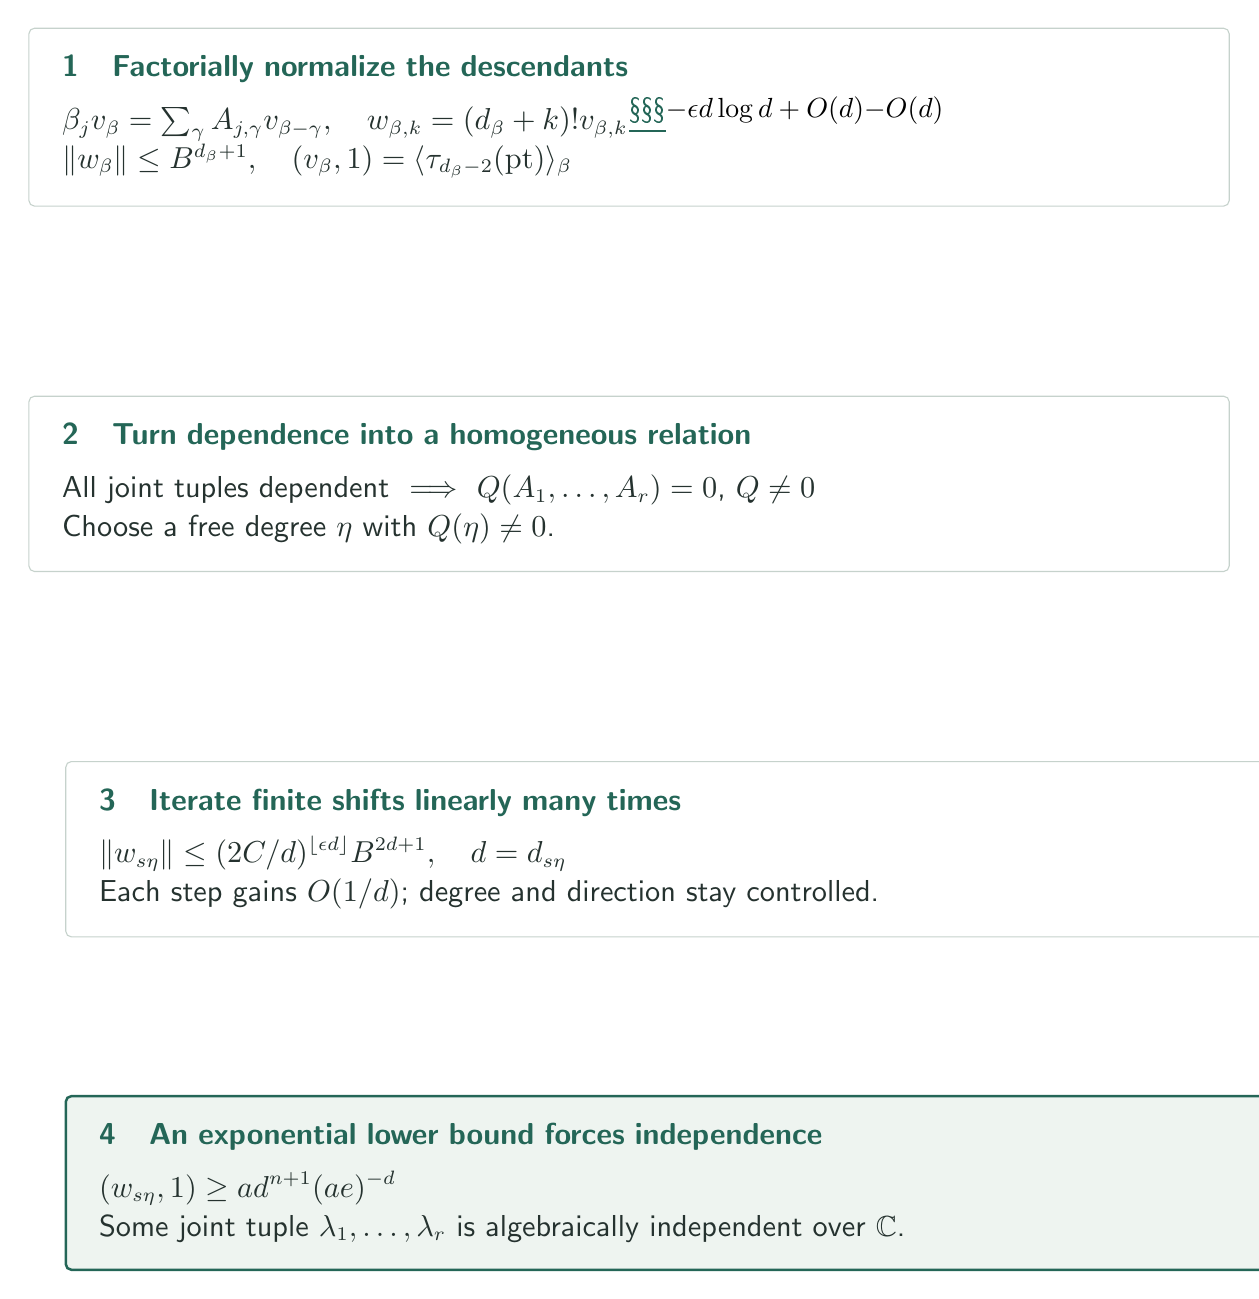
\begin{tikzpicture}

\node[card] (a) {\heading{1}{descendant を階乗正規化}{Factorially normalize the descendants}
$\beta_jv_\beta=\sum_\gamma A_{j,\gamma}v_{\beta-\gamma},\quad
w_{\beta,k}=(d_\beta+k)!v_{\beta,k}$\\
$\|w_\beta\|\le B^{d_\beta+1},\quad (v_\beta,1)=\langle\tau_{d_\beta-2}(\mathrm{pt})\rangle_\beta$};
\node[card,below=2.4cm of a] (b) {\heading{2}{従属性から斉次関係式を作る}{Turn dependence into a homogeneous relation}
\Tx{全 joint tuple が従属 $\ \Longrightarrow\ Q(A_1,\ldots,A_r)=0$, $Q\ne0$}{All joint tuples dependent $\ \Longrightarrow\ Q(A_1,\ldots,A_r)=0$, $Q\ne0$}\\
\Tx{free な $\eta$ を $Q(\eta)\ne0$ となるよう選ぶ}{Choose a free degree $\eta$ with $Q(\eta)\ne0$.}};
\flow{a}{b}{\PRef{Lemma 2.1; \S4.1, pp. 5, 11--12}\ \Tx{（漸化式・指数上界）}{(recurrence; exponential bound)}\\
\KMRef{Correlator relations, Lemma 1.4}\ +\ \PARef{Rational curves on hypersurfaces, \S1.2}\\
\Tx{斉次化と free 次数の稠密性：}{Homogeneity and density of free degrees: }\PRef{Lemma 3.3; \S4.2, pp. 10--12}};
\node[card,below=2.4cm of b] (c) {\heading{3}{有限シフトを線形回数だけ反復}{Iterate finite shifts linearly many times}
$\displaystyle\|w_{s\eta}\|\le(2C/d)^{\lfloor\epsilon d\rfloor}B^{2d+1},\quad d=d_{s\eta}$\\
\Tx{各段で $O(1/d)$、$\lfloor\epsilon d\rfloor$ 回の間は次数と方向を制御}{Each step gains $O(1/d)$; degree and direction stay controlled.}};
\flow{b}{c}{\TZRef{One-cycles, Thm. 1.3; Prop. 2.4}\ \Tx{（生成・comb smoothing）}{(generation; comb smoothing)}\\
\Tx{多項式差分と有限シフト：}{Polynomial differences and finite shifts: }\PRef{(9)--(11), pp. 12--13}};
\node[result,below=2cm of c] (d) {\heading{4}{指数下界との矛盾で独立性を得る}{An exponential lower bound forces independence}
$\displaystyle (w_{s\eta},1)\ge a d^{n+1}(ae)^{-d}$\\
\Tx{ある joint tuple $\lambda_1,\ldots,\lambda_r$ は $\mathbb C$ 上代数的独立}{Some joint tuple $\lambda_1,\ldots,\lambda_r$ is algebraically independent over $\mathbb C$.}};
\flow{c}{d}{\Tx{上界の対数 $-\epsilon d\log d+O(d)$ と下界 $-O(d)$ が矛盾：}{Logarithms $-\epsilon d\log d+O(d)$ and $-O(d)$ contradict each other:}\\
\PRef{Prop. 3.1; Prop. 4.1, pp. 6, 13}};

\end{tikzpicture}
\end{document}
